\documentclass[10pt]{article}
\usepackage[margin=1in]{geometry}
\usepackage{graphicx}
\usepackage{fancyhdr}
\usepackage{calc}
\usepackage{amsmath}
\usepackage{float}
\pagestyle{fancy}
\fancyhf{}
\setcounter{secnumdepth}{-1}

\begin{document}

\title{198:416 A02}
\author{Eric Cuiffo, Nick Palumbo, Val A. Red, Aiser Sheikh}

\fancyhead{}
\fancyhead[LO]{\bfseries Eric Cuiffo, Nick Palumbo, Val A. Red, Aiser Sheikh}
\fancyhead[RO]{198:416 A02 Fair Share Scheduler}
\hspace*{95pt} $\spadesuit$\\
Eric Cuiffo, Nick Palumbo, Val A. Red, Aiser Sheikh\\
27 March 2013 \\
198:416 Operating Systems, A02.
\section{Fair Share Scheduler}
I. Introduction \\
II. Areas of Change \\
III. Imeplementation Details \\
IV. Overhead \\
V.  Testing \\
VI. Further improvement

\section{I. Introduction:}

Our group (incorporating Eric Cuiffo, Nick Palumbo, Val A. Red, and Aiser Sheikh) implemented a fair 
share scheduler in the Linux 2.4.24 kernel via a provided debian distribution. 
All user's processes will share an equal portion of CPU time in a way such that one
user cannot use another user's equal portion. In addition, we implemented a system call
that enables a user to request a double share to be allocated for its process. We called
our system call \texttt{incshare.} \\* \\*
\hspace*{36pt} Our \texttt{patch\_name.patch} file can be deployed in the Linux-2.4.24 directory via the following command \\*
\begin{verbatim}
patch -p1 -i patch_name.patch
\end{verbatim}

Data gathered from our implementation will be discussed in this report. We deployed on the
Rutgers' Computer Science department's iLab Computers. 

\section{Invoking incshare()}
We named our system call \texttt{incshare} instead of myincshare. It can be defined as followed: 
\begin{verbatim}
12         #define __NR_incshare 259
13         _syscall0(int, incshare);
.
.
.
51        incshare()
\end{verbatim}

\section{II. Areas of Change:}

Our modification of the kernel was mainly aimed at the files involved with the scheduler, with one addition of a system call, (\texttt{inchsare}. ) Overall, we added lines to the scheduling files to implement an algorithm that was a Fair Share Scheduler; essentially enabling multiple users logged into the machine to receive an equal allocation of CPU time for their processes. \\ \\

The addition of the system call, \texttt{incshare()} also allowed users to give one of their processes a greater subdivision of CPU time out of their own allocation. \\* \\* \\*

--- {\bfseries As an overview, our \texttt{patch\_name.patch} has edited the following files in the kernel:}
\begin{verbatim}
      arch/i386/kernel/entry.S
      include/asm-i386/unistd.h
      include/linux/sched.h
      kernel/exit.c
      kernel/fork.c
      kernel/sched.c
      kernel/sys.c                       // Where incshare() is implemented and defined
      Makefile
\end{verbatim}
--- {\bfseries To the process struct, we added} \texttt{atomic\_t share}. \\* \\*
\hspace*{36pt} This keeps track of how many times our system call \texttt{incshare} was
called on a process; \\ 
\hspace*{36pt} initializes as ``1'' by default. \\* \\* 
--- {\bfseries Added the initialization of \texttt{p-\textgreater share} to 1 in do\_fork} \\* \\*
--- {\bfseries On each repeat schedule, we counted number of processes (using for\_each\_task)}


\section{III. Implementation Details:}

In the \texttt{task\_struct} (which represents a process) there is a field called \texttt{counter}. In the original implementation of the Linux scheduler, this is initialized to the niceness value for a CPU-bound process. (For I/O bound processes, the previous counter value is taken into consideration and shifted right—For CPU-bound processes, the counter value reaches 0 before re-initialization.) As we are assuming all CPU-bound processes, the counter values will not be reinitialized until all the processes' counters have reached 0 (technically only processes on the run queue, but we are assuming no blocking, so all processes should be on the run queue).

In order to implement the per-user scheduling algorithm defined in the assignment, we need to manipulate the value the counter is initialized to. Because the counter is decremented by one each time a process is scheduled, the ratio of initial counter values will correspond to the ratio of CPU time each process gets. (For example, if one process has a counter value of 5 and one has a counter value of 10, the second process will get twice as much CPU time before a re-initialization occurs).

Thus, in order to implement the desired scheduling, we initialized the counter for each process to the following calculation:

counter$ = \frac{\text{total number procs}}{\text{this user's number of procs}}$ \\
We can prove that this gives each user the same total amount of CPU time:

This equation ensures that each user's collective counter total for their processes will be equal to the total number of processes in the system. If all their collective counter totals are equal, then each user is getting the same amount of process time. We can also observe that users with more processes will get less CPU time per process. In addition, each of a user's processes (in the absence of a system call) will get the same CPU Time. This is congruent with our desired behavior. We also ensure that if this would result in a counter value of 0 for a process, we instead initialize it to 1.

Finally, in order to implement the system call, we used an \texttt{atomic\_t} called share is the task\_struct. When a process calls incshare, the share value increases from 1 to 2. In addition, the number of processes a user has is artificially increased by 1. We ensured that when a process that has called the incshare exits, the user's number of processes is decreased by 2 to maintain consistency. The calculation for counter initialization is altered:

counter$ = \text{share}\frac{\text{total number procs}}{\text{this user's number of procs}}$

It is clear that if no process calls incshare, the desired behavior is still observed. If a process calls incshare, it is clear that only that user's processes have their counter's altered and that process will get twice as much as the other process for that user.

{\textit{Defining the system call via \textbf{entry.S}, \textbf{unistd.h}, and \textbf{sys.c} :}} \\

We first needed to define our system-call handling routine via the Entry.s file. We accomplished this by adding the following to linux/arch/i386/kernel/entry.S \\

\begin{verbatim}
666                           .long SYMBOL_NAME(sys_incshare)
\end{verbatim}

{\textit{Adding a unistd.h entry and wrapper function}}

We then added an entry to include/asm-i386/unistd.h and proceeded to add our wrapper function:
\begin{verbatim}
260                           #define __NR_incshare        259
 .
 .
 .
379                           static inline _syscall0(int,incshare)
\end{verbatim}

Finally, we decided that we would add our system call through sys.c. In order to do this, we added the following lines to /kernel/sys.c :
\begin{verbatim}
1288                          asmlinkage int sys incshare()
1289                          {
 .
 .
 .
1300                          }
\end{verbatim}

\section{IV. Overhead:}

The overhead generated by our changes includes the time it takes to calculate the the total number of processes (which is equivalent to the time it takes to step through the processes in for\_each\_task and the time it takes to increment an integer). Also, the time it takes to initialize the atomic\_t share when a process is created in fork. With regards to space, we are storing an addition atomic\_t per process. Thus, we are using sizeof(\texttt{atomic\_t}) additional space per process.

\section{V. Testing:}
\begin{figure}[H]
 \caption{Sample text}
 \centering
 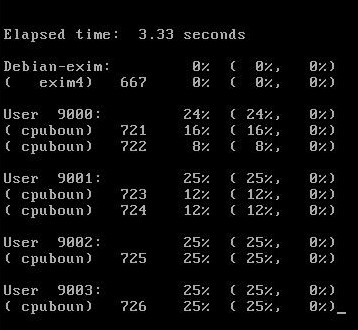
\includegraphics[width=250px]{incsharemonitor.jpg}
\end{figure}


\section{VI. Further improvement:}

Our \texttt{for\_each\_task} does not necessarily count every single process that exists in the system (we believe processes that do things w/r/t the kernel are not being counted, things such as init). However, our project is only concerned with the processes that we have control over and does not need to worry about the scheduling of those low-level processes. This may, however, cause a few percent discrepancy for CPU time in different processes. It may be worth at some point looking into a more accurate or quicker way to determine the number of processes in the system. In addition, as our implementation using a little extra space per process, it may limit the total number of processes that can be in the system than usual--more resources as being used. Finally, in the presence of many I/O bound processes, our algorithm will fail. The counter values we used are only appropriate for CPU bound processes and will be inaccurate for I/O bound processes. However, our project operated under the assumption of only CPU-bound processes.


\end{document}
